% % -----------------------------------------------------------------------------
\section{Overview of OPIL}
% % -----------------------------------------------------------------------------

In OPIL, a protocol is an activity that is configured with certain parameters and applied to a set of biological samples in order to produce a set of measurements by particular instruments at particular times, as illustrated in \ref{f:overview}.
An \opil{ExperimentalRequest} specifies a particular set of \opil{ParameterValue}s, \opil{SampleSet}s, and \opil{Measurement}s to be carried out. 
A \opil{ProtocolInterface} specifies which \opil{ExperimentalRequest}s are allowed for a given protocol with a parallel construction of \opil{Parameter}s, \opil{SampleSet}s, and \opil{MeasurementType}s

\begin{figure}[ht]
\begin{center}
  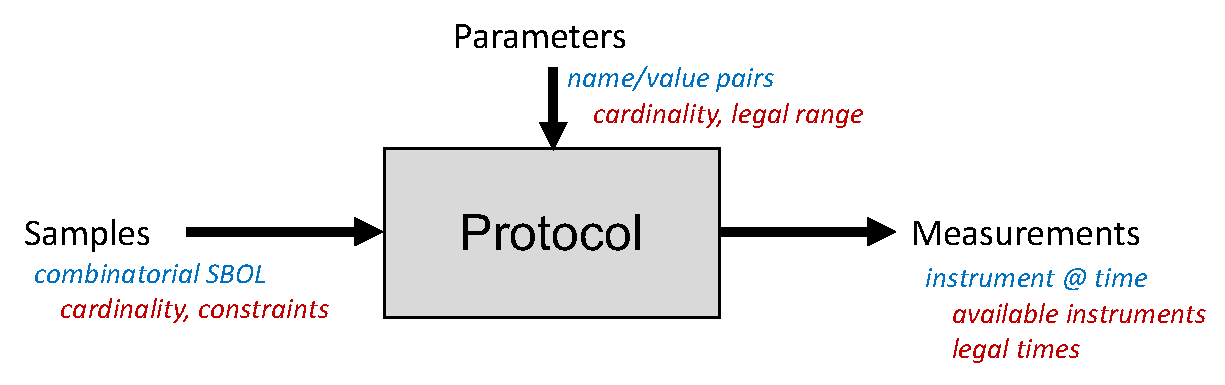
\includegraphics[scale=0.75]{figures/overview.pdf}
\caption{OPIL describes a request (blue) to execute a protocol in terms of samples, parameters, and measurements. 
A protocol interface (red) specifies what sorts of execution requests are allowed for that protocol.}
\label{f:overview}
\end{center}
\end{figure}

For example, consider a lab that is offering a multi-day bacterial protocol that might be described in prose as follows:
\begin{quote}
``Run either B. subtilis or E. coli samples in any media with up to 2 inducers for 1 to 4 days, sampling with a flow cytometer no more than once every 12 hours, and have the option of taking one RNAseq measurement. Culturing temperature is normally 37 C but can be set anywhere between 20 and 40 C.''
\end{quote}
These constraints could be encoded into a \opil{ProtocolInterface} by dividing them up as follows:
\begin{itemize}
\item Using \opil{SampleSet} objects: any {\it B. subtilis} or {\it E. coli} strain in any media, with up to 2 inducers.
\item Using \opil{Parameter} objects: run for 1-4 days, culture between 20-40 C with a default of 37 C.
\item Using \opil{MeasurementType} objects: any number of flow cytometer samples at least 12 hours apart, zero or one RNAseq measurement at any time.
\end{itemize}

An experimentalist who wishes to use this protocol might want to make a request such as the following:
\begin{quote}
``Please run all combinations of strains X and Y in media A, B, and C with 0, 0.1, 0.2, 0.5, and 1.0 uM arabinose. Run for 3 days with flow cytometry at hours 12, 30, 48, and 70. Culture at 27 C.''
\end{quote}
These specifies could be encoded into an \opil{ExperimentalRequest} by dividing them up as follows:
\begin{itemize}
\item Using \opil{SampleSet} objects: all combinations of strains X and Y in media A, B, and C with 0, 0.1, 0.2, 0.5, and 1.0 uM arabinose.
\item Using \opil{ParameterValue} objects: run for 3 days, culture at 27 C.
\item Using \opil{Measurement} objects: flow cytometry at hours 12, 30, 48, and 70.
\end{itemize}

The next sections provide complete definitions and details for all of these classes, along with more examples of their use.
